\documentclass{article}
\usepackage[margin=2.5cm]{geometry} % Set margins
\usepackage{graphicx}
\usepackage[absolute]{textpos} % Enable absolute positioning
\usepackage{titlesec} % Package for controlling section title appearance
\usepackage[scaled]{helvet}
\usepackage[T1]{fontenc}
\usepackage{fancyhdr}
\usepackage[utf8]{inputenc}
\usepackage{lmodern}
\usepackage{amsmath}
\usepackage{url} % Load the url package

% Set up colors
\usepackage[dvipsnames]{xcolor} % Color management
% ZHAW Blue: Pantone 2945 U / R0 G100 B166
\definecolor{zhawblue}{rgb}{0.00, 0.39, 0.65}
\definecolor{zhawlightblue}{rgb}{0.82, 0.88, 0.93}

% Set up hyperref
\usepackage{hyperref}
\hypersetup{
    colorlinks=true,
    linkcolor=zhawblue,
    urlcolor=zhawblue,
    citecolor=zhawblue,
    linkbordercolor={0 0 1}
}

% Set up references
\usepackage[
    backend=biber,             % Use biber backend (an external tool)
    sorting=nyt,              % Enumerates the reference in order of their appearance
    style=apa          % Choose here your preferred citation style
]{biblatex}
\addbibresource{../../biblatex_ba.bib} % The filename of the bibliography

\usepackage[english]{babel} % Set the document language to English

\usepackage[autostyle=true, english=american]{csquotes} 
                               % Required to generate language-dependent quotes 
                               % in the bibliography

\setlength{\TPHorizModule}{1cm} % Set horizontal unit of measure
\setlength{\TPVertModule}{1cm} % Set vertical unit of measure
\setlength{\parindent}{0pt}

\renewcommand{\familydefault}{\sfdefault}

\makeatletter
\renewcommand{\maketitle}{
  \begin{flushleft} 
    \Large\textmd{\@title} 
    \par
  \end{flushleft}
}
\makeatother

% Define style of sectiontitles
\titleformat{\section}
  {\normalfont\large\mdseries}{\thesection}{1em}{}

\titleformat{\subsection}
  {\normalfont\normalsize\itshape} % Adjust style: smaller size, italic
  {} % No label
  {0pt} % Spacing between label and title
  {} % Code to execute after the title
\titlespacing*{\subsection}
  {0pt} % Left margin
  {0.8em} % Space above
  {0.2em} % Space below

% Set up fancyhdr
\fancyhf{} % Clear all headers and footers
\renewcommand{\headrulewidth}{0pt} % Remove the header rule
\rfoot{\thepage} % Place the page number in the right footer
\pagestyle{fancy}

% Add listings package for code highlighting
\usepackage{listings}
\usepackage{xcolor}

%%%%% Title %%%%%
\title{Proposed Workflow for Sequential Based Species Classification of Camera Trap Images}

\begin{document}

%%%%% Header %%%%%
\begin{textblock}{5}(2.5,1) % Position 1cm from left and 1cm from top
  
\includegraphics[width=5cm]{resources/logo.jpg} % Add logo
\end{textblock}

\begin{textblock}{6}(13,1) % Position 14cm from left and 1cm from top
        \raggedleft
        Julian Kraft UI22\\
        Proposed Workflow V2\\
        \today
\end{textblock}

\vspace*{1.5cm}

%%%%% Document %%%%%

\maketitle

%%%%%   %%%%%

\section*{Situation} %%%%%%%%%%%%%%%%%%%%%%%%%%%%%%%%%%%%%%%%%%%%%%%%%%%%%%%%%%%%%%%%%%%%%%%%%%%%%%%%%%%%%%%%%%%%%%%%%%%

The project Wildlife@Campus is a project of the ZHAW and aims to monitor small mustelids in Switzerland.
One approach of the project is using camera traps to collect images of the animals. 
The images are taken using a camera trap box called MammaliaBox especially adapted for this
project \autocite{grafWildlifeCampusKleineSaeugetiere2022}.
The use of cameratraps for wildlifemonitoring is an well established method 
\autocite{cordierCameraTrapResearch2022, beaudrotStandardizedAssessmentBiodiversity2016}. 
Evaluating the large amount of data collected by cameratraps
is providing a resource heavy task -- especially if approached manually. The use of machine learning algorithms 
have proven to be a valuable tool for minimizing the workload. There are several approaches to classify and species and
to detect animals in images \autocite{tabakMachineLearningClassify2019, bohnerSemiautomaticWorkflowProcess2023}. 
While the most common approach is to classify single images, for this project a sequential based approach is tested.

\section*{Dataset} %%%%%%%%%%%%%%%%%%%%%%%%%%%%%%%%%%%%%%%%%%%%%%%%%%%%%%%%%%%%%%%%%%%%%%%%%%%%%%%%%%%%%%%%%%%%%%%%%%%%%%

As part of the Wildlife@Campus project a labeled dataset was created to train a deep learning algorithm.
The dataset is divided into 7 sessions. The images are grouped into sequences of images taken of the same sighting 
of an animal. The sequences are not of a standardized length and can vary from 1 to 915 files per sequence.
There is to mention that in a later use case this sequence length will most likely be more standardized.
The actual length will depend on the camera setting -- common settings are 1, 3, 5 or 10 images per trigger -- 
can be extracted from the EXIF information of the images. The dataset provides two types of labels for the sequences 
the second one is a simplified and standardized version of the labels. For this project only the simplified version 
will be used. The distribution of the available sequences per label is shown in \autoref{fig:sequenceperlabel}.
The category \texttt{other} represents sequences containing more than one species the category \texttt{NaN} 
represents sequences without a label -- both will be excluded from the training data. 
The category \texttt{glis\_glis} is only represented in 4 sequences -- a challenge to be addressed.
20\% of the sequences will be used for testing only a stratified split will be done with a fixed seed to ensure
reproducibility.

\begin{figure}[ht]
  \centering
  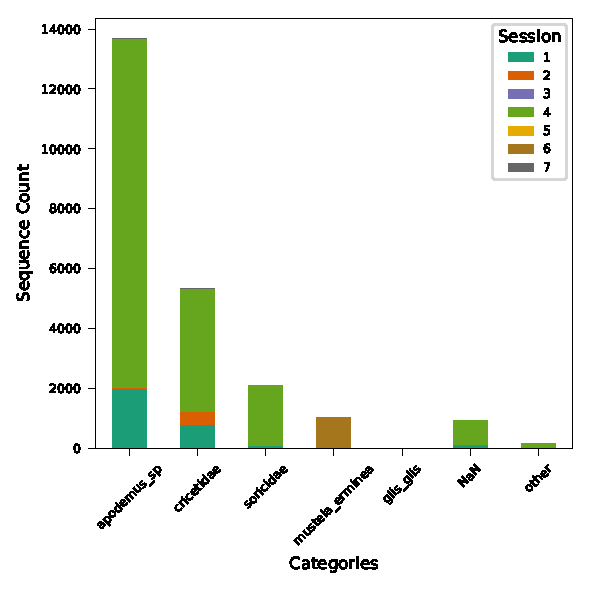
\includegraphics{resources/label2_session.pdf}
  \caption{Available sequences per label colored by session.}
  \label{fig:sequenceperlabel}
\end{figure}

\section*{General Idea for the Model} %%%%%%%%%%%%%%%%%%%%%%%%%%%%%%%%%%%%%%%%%%%%%%%%%%%%%%%%%%%%%%%%%%%%%%%%%%%%%%%%%%

The general idea is to create a Model that can classify the species of a sequence of images utilizing all the relevant 
areas of all the images. So the model needs to be able to handle a sequence of input images that can vary in length. 
This will be achieved by processing all the relevant areas individually and extract a standardized feature array from 
each area. This feature arrays will be combined into one using average pooling. This combined feature array
will be feed into a final fully connected layer to classify the species.

\section*{Data Preparation} %%%%%%%%%%%%%%%%%%%%%%%%%%%%%%%%%%%%%%%%%%%%%%%%%%%%%%%%%%%%%%%%%%%%%%%%%%%%%%%%%%%%%%%%%%%%%

The Microsoft MegaDetector (MD) is a well established model for detecting animals in camera trap images 
\autocite{hernandezPytorchWildlifeCollaborativeDeep2024a, velezChoosingAppropriatePlatform2022, 
schneiderRecognitionEuropeanMammals2024}. In this project the MD will be used to detect the animals in all the images
of every sequence. The MD outputs a list of bounding boxes for detected animals, humans and vehicles 
and a corresponding confidence scores. All bounding boxes for animals with a confidence score above a certain threshold 
-- possibly 0.5 -- of a sequence will be extracted and used for classification. This areas will be resized to a fixed 
size -- 224 x 224 pixels -- as this is the size ResNet50 expects. For the training the data will be augmented 
using random rotation and random flip -- arguably the most simple augmentation techniques for images.

\section*{Model Architecture} %%%%%%%%%%%%%%%%%%%%%%%%%%%%%%%%%%%%%%%%%%%%%%%%%%%%%%%%%%%%%%%%%%%%%%%%%%%%%%%%%%%%%%%%%%%%

The proposed model architecture is shown in \autoref{fig:model}. The idea is to use a pretrained ResNet50 model to 
extract features from the images. This is a well established model that has proven to work well for image classification 
tasks. The model will be used to extract features from the selected areas of the images. The features will be embedded 
into a feature array of a fixed length. To achieve this the last layer of the ResNet50 will be customized slightly. 
A reasonable number of features to extract is still to be determined. This n arrays will be combined into one using 
average pooling. This is a the simples possible way to combine this features while standardizing the shape for the input 
to the final fully connected layer predicting the species.

\begin{figure}[ht]
  \centering
  \includegraphics{resources/model_proposal.pdf}
  \caption{Visual representation of the proposed model architecture.}
  \label{fig:model}
\end{figure}

\section*{Training} %%%%%%%%%%%%%%%%%%%%%%%%%%%%%%%%%%%%%%%%%%%%%%%%%%%%%%%%%%%%%%%%%%%%%%%%%%%%%%%%%%%%%%%%%%%%%%%%%%%%%%

For the training the plan is to fixe the size of the input for optimal performance. To avoid the model getting used to 
fixed sequence length and to maximise input variety for a robust model a batch will be created by two parameters: 
The number of sequences and the mean number of images per sequence. The number of images will than be randomly 
distributed among the sequences. From each sequence the assigned number of images will be randomly sampled
from the available images allowing for repetition to avoid issues with sequences with less images than the 
assigned number and to further increase the variety of the input. The pretrained ResNet50 model will be frozen and only 
the last -- customized layer will be trained. The model will be trained using a cross entropy loss function and the 
Adam optimizer.

\section*{Hyperparemeter Tuning and Cross Validation} %%%%%%%%%%%%%%%%%%%%%%%%%%%%%%%%%%%%%%%%%%%%%%%%%%%%%%%%%%%%%%%%%%%%

A first stratified 80/20 split will be done to perform a hyperparameter tuning with a grid search using the validation
set for an early stopping routine. Using the best hyperparameters a 5 fold cross validation will be performed to
evaluate the model performance.

\section*{Prediction} %%%%%%%%%%%%%%%%%%%%%%%%%%%%%%%%%%%%%%%%%%%%%%%%%%%%%%%%%%%%%%%%%%%%%%%%%%%%%%%%%%%%%%%%%%%%%%%%%%%%

On each training compleation, the best performing model will be loaded and the test set will be predicted. 
For the prediction the approach is slightly changed. All the relevant areas of the images will be feed into the model 
instead of sampling a random number of them and the data augmentation will not be used. 
This is to ensure all available information is used for the prediction. Since some of the sequences in the available 
dataset are quite long some kind of limit might be needed to avoid memory issues.

%%%%%%%%%%%%%%%%%%%%%%%%%%%%%%%%%%%%%%%%%%%%%%%%%%%%%%%%%%%%%%%%%%%%%%%%%%%%%%%%%%%%%%%%%%%%%%%%%%%%%%%%%%%%%%%%%%%%%%%%%

\printbibliography

\end{document}
